% THIS IS SIGPROC-SP.TEX - VERSION 3.1
% WORKS WITH V3.2SP OF ACM_PROC_ARTICLE-SP.CLS
% APRIL 2009
%
% It is an example file showing how to use the 'acm_proc_article-sp.cls' V3.2SP
% LaTeX2e document class file for Conference Proceedings submissions.
% ----------------------------------------------------------------------------------------------------------------
% This .tex file (and associated .cls V3.2SP) *DOES NOT* produce:
%       1) The Permission Statement
%       2) The Conference (location) Info information
%       3) The Copyright Line with ACM data
%       4) Page numbering
% ---------------------------------------------------------------------------------------------------------------
% It is an example which *does* use the .bib file (from which the .bbl file
% is produced).
% REMEMBER HOWEVER: After having produced the .bbl file,
% and prior to final submission,
% you need to 'insert'  your .bbl file into your source .tex file so as to provide
% ONE 'self-contained' source file.
%
% Questions regarding SIGS should be sent to
% Adrienne Griscti ---> griscti@acm.org
%
% Questions/suggestions regarding the guidelines, .tex and .cls files, etc. to
% Gerald Murray ---> murray@hq.acm.org
%
% For tracking purposes - this is V3.1SP - APRIL 2009

\documentclass{edm_article}

\usepackage{bm}

\begin{document}

\title{The Effect of an Intelligent Tutor on Performance on Specific Posttest Problems}
%\subtitle{[Extended Abstract]
%\titlenote{A full version of this paper is available as
%\textit{Author's Guide to Preparing ACM SIG Proceedings Using
%\LaTeX$2_\epsilon$\ and BibTeX} at
%\texttt{www.acm.org/eaddress.htm}}}
%
% Submissions for EDM are double-blind: please do not include any
% author names or affiliations in the submission. 
% Anonymous authors:

% \numberofauthors{8} %  in this sample file, there are a *total*
% % of EIGHT authors. SIX appear on the 'first-page' (for formatting
% % reasons) and the remaining two appear in the \additionalauthors section.
% %
% \author{
% % You can go ahead and credit any number of authors here,
% % e.g. one 'row of three' or two rows (consisting of one row of three
% % and a second row of one, two or three).
% %
% % The command \alignauthor (no curly braces needed) should
% % precede each author name, affiliation/snail-mail address and
% % e-mail address. Additionally, tag each line of
% % affiliation/address with \affaddr, and tag the
% % e-mail address with \email.
% %
% % 1st. author
% \alignauthor
% Ben Trovato\titlenote{Dr.~Trovato insisted his name be first.}\\
%        \affaddr{Institute for Clarity in Documentation}\\
%        \affaddr{1932 Wallamaloo Lane}\\
%        \affaddr{Wallamaloo, New Zealand}\\
%        \email{trovato@corporation.com}
% % 2nd. author
% \alignauthor
% G.K.M. Tobin\titlenote{The secretary disavows
% any knowledge of this author's actions.}\\
%        \affaddr{Institute for Clarity in Documentation}\\
%        \affaddr{P.O. Box 1212}\\
%        \affaddr{Dublin, Ohio 43017-6221}\\
%        \email{webmaster@marysville-ohio.com}
% % 3rd. author
% \alignauthor Lars Th{\o}rv{\"a}ld\titlenote{This author is the
% one who did all the really hard work.}\\
%        \affaddr{The Th{\o}rv{\"a}ld Group}\\
%        \affaddr{1 Th{\o}rv{\"a}ld Circle}\\
%        \affaddr{Hekla, Iceland}\\
%        \email{larst@affiliation.org}
% \and  % use '\and' if you need 'another row' of author names
% % 4th. author
% \alignauthor Lawrence P. Leipuner\\
%        \affaddr{Brookhaven Laboratories}\\
%        \affaddr{Brookhaven National Lab}\\
%        \affaddr{P.O. Box 5000}\\
%        \email{lleipuner@researchlabs.org}
% % 5th. author
% \alignauthor Sean Fogarty\\
%        \affaddr{NASA Ames Research Center}\\
%        \affaddr{Moffett Field}\\
%        \affaddr{California 94035}\\
%        \email{fogartys@amesres.org}
% % 6th. author
% \alignauthor Charles Palmer\\
%        \affaddr{Palmer Research Laboratories}\\
%        \affaddr{8600 Datapoint Drive}\\
%        \affaddr{San Antonio, Texas 78229}\\
%        \email{cpalmer@prl.com}
% }
% % There's nothing stopping you putting the seventh, eighth, etc.
% % author on the opening page (as the 'third row') but we ask,
% % for aesthetic reasons that you place these 'additional authors'
% % in the \additional authors block, viz.
% \additionalauthors{Additional authors: John Smith (The Th{\o}rv{\"a}ld Group,
% email: {\texttt{jsmith@affiliation.org}}) and Julius P.~Kumquat
% (The Kumquat Consortium, email: {\texttt{jpkumquat@consortium.net}}).}
% \date{30 July 1999}
% Just remember to make sure that the TOTAL number of authors
% is the number that will appear on the first page PLUS the
% number that will appear in the \additionalauthors section.

\maketitle

%\onecolumn


\begin{abstract}
This paper drills deeper into the documented effects of the Cognitive Tutor Algebra I and ASSISTments intelligent tutoring systems by estimating their effects on specific problems. We start by describing a multilevel Rasch-type model that facilitates testing for differences in the effects between problems and precise problem-specific effect estimation without the need for multiple comparisons corrections. We find that the effects of both intelligent tutors vary between problems--the effects are positive for some, negative for others, and undeterminable for the rest. Next we explore hypotheses explaining why effects might be larger for some problems than for others. In the case of ASSISTments, there is no evidence that problems that are more closely related to students' work in the tutor displayed larger treatment effects.
\end{abstract}

%% A category with the (minimum) three required fields
%\category{H.4}{Information Systems Applications}{Miscellaneous}
%%A category including the fourth, optional field follows...
%\category{D.2.8}{Software Engineering}{Metrics}[complexity measures, performance measures]
%
%\terms{Theory}

\keywords{Causal impact estimates,multilevel modeling,intelligent tutoring systems}

\section{Introduction: Average and Item-Specific Effects}

The past decade has seen increasing evidence of the effectiveness of
intelligent tutoring systems (ITS) in supporting student learning \cite{escueta2017education}\cite{kulik2016effectiveness}.
However, surprisingly little detail is known about these
effects such as which students experience the biggest benefits, under what conditions.
This paper will focus on the question of which areas of learning 
had the largest impact in two different year-long randomized trials: of the
Cognitive Tutor Algebra I curriculum (CTA1) \cite{pane2014effectiveness} and
of the ASSISTments ITS \cite{roschelle2016online}.

Large-scale efficacy or effectiveness trials in education research,
including evaluations of ITS
\cite{pane2014effectiveness}\cite{pane2010experiment}\cite{roschelle2016online},
often estimate the effect of an educational intervention on student
scores on a standardized test.
These tests consist of many items, each of which tests student
abilities in, potentially, a separate set of skills.
Prior to estimating program effects, analysts collapse data across
items into student scores, often using item response theory models
\cite{van2013handbook} that measure both item- and student-level
parameters. 
Then, these student scores are compared between students assigned to
the intervention group and those assigned to control.

This approach has its advantages, in terms of simplicity and (at least
after aggregating item data into test scores) model-free causal
identification. 
If each item is a measurement of one underlying latent construct (such
as ``algebra ability'') aggregating items into test scores yields
efficiency gains. 
However, in the (quite plausible) case that posttest items actually
measure different skills, and the impact of the ITS varies from skill
to skill, item-specific impacts can be quite informative.

In the case of CTA1 and ASSISTments, we find that, indeed, the ITS
affect student performance differently on different posttest items,
though at this stage it is unclear why the affects differed. 

The following section gives an overview of the two large-scale ITS
evaluations we will discuss, including a discussion of the available
data and of the two posttests. Next, Section~\ref{sec:method} will
discuss the Bayesian multilevel model we use to estimate item-specific
effects, including a discussion of multiple comparisons;
Section~\ref{sec:results} will discuss the results---estimates of how
the two ITS impacted different posttest items differently;
Section~\ref{sec:hypotheses} will present a preliminary exploration of
some hypotheses as to why ASSISTments may have impacted different
skills differently; and Section~\ref{sec:conclusion} will conclude.


\section{The CTA1 and ASSISTments Trials}
This paper uses data from two large-scale field trials of ITSs CTA1
and ASSISTments. The CTA1 intervention consisted of a complete curriculum,
combining the Cognitive Tutor ITS, along with a student-centered
classroom curriculum. CTA1 was a created and run by Carnegie Learning;
an updated version of the ITS is now known as Mathia. The Cognitive
Tutor is described in more detail in \cite{anderson1995cognitive} and
elsewhere, and the effectiveness trial is described in \cite{pane2014effectiveness}.
ASSISTments is a free online-homework platform, hosted by Worcester
Polytechnic Institute, that combines electronic versions of textbook
problems, including on-demand hints and immediate feedback, with
bespoke mastery-based problem sets known as ``skill builders.''
ASSISTments is described in \cite{heffernan2014assistments} and the
efficacy trial is described in \cite{roschelle2016online}.

This section describes the essential aspects of the field trials and
the data that we will use in the rest of the paper. 

\subsection{The CTA1 Effectiveness Trial}
From 2007 to 2010, the RAND Corporation conducted a randomized
controlled trial to compare the effectiveness of the CTA1 curriculum
to business as usual (BaU). The study tested CTA1 under authentic, natural
conditions, i.e., oversight and support of CTA1's use was the same as
it would have been if there was not a study being conducted. Nearly
20,000 students in 70 high schools ($n=13,316$ students) and 76 middle
schools ($n=5,938$) located in 52
diverse school districts in seven states participated in the
study. Participating students in Algebra I classrooms took an algebra
I pretest and a posttest, both from the CTB/McGraw-Hill Acuity series. 

Schools were blocked into pairs prior to
randomization, based on a set baseline, school-level covariates, and
within each pair, one school was assigned to the CTA1 
arm and the other to BaU.
In the treatment schools, students taking algebra I were supposed to
use the CTA1 curriculum, including the Cognitive Tutor software; of
course, the extent of compliance varied widely
\cite{karam2017examining}\cite{descriptivePaper}. 

Results from the first and second year of the study were reported
separately for middle and high schools. In the first year, the
estimated treatment effect was close to zero in middle schools and
slightly negative in high schools. However, the 95\% confidence
intervals for both these results included negative, null, and positive
effects. In the second year, the estimated treatment effect was
positive--roughly one fifth of a standard deviation---for both middle
and high schools, but it was only statistically significant in the
high school stratum.

In this study, we make use of students' overall scores on the pretest,
anonymized student, teacher, school, and randomization block IDs, and
an indicator variable for whether each student's school was assigned
to the CTA1 or BaU, along with item-level posttest data: whether each
student answered each posttest item correctly.
For the purposes of this study, skipped items were considered
incorrect. 

\subsubsection{Posttest: The Algebra Proficiency Exam}
The RAND CTA1 study measured the algebra I learning over the course of
the year using the McGraw-Hill Algebra Proficiency Exam (APE). 
This was a multiple choice standardized test with 32 items testing
a mix of algebra and pre-algebra skills.
Table \ref{tab:ctSkills}, categorizes the test's items by the algebra
skills they require, and gives an example of a problem that would fall
into each category.
The categorization was taken from the exam's technical report
\cite{ctTechReport}.


% latex table generated in R 4.0.3 by xtable 1.8-4 package
% Wed Mar 03 18:49:16 2021
\begin{table*}[ht]
\centering
\begin{tabular}{p{2.5in}p{1in}p{2.5in}}
  \hline
Objective & Items & Example \\ 
  \hline
Functions and Graphs & 6, 8, 19, 20, 22, 23, 27, 31, 32 & Which of these points is on the graph of [function] \\ 
  Geometry & 12, 18, 24, 29 & Find the length of the base of the right triangle shown below \\ 
  Graphing Linear Equations & 5, 9, 15, 17, 26 & Which of the lines below is the graph of [linear equation]? \\ 
  Quadratic Equations and Functions & 2, 25, 28, 30 & Which of these shows a correct factorization of [quadratic equation]? \\ 
  Solving Linear Equations and Linear Inequalities & 1, 4, 11, 13, 16 & Solve the following system of equations \\ 
  Variables, Expressions, Formulas & 3, 7, 10, 14, 21 & Which of these expressions is equivalent to the one below? \\ 
   \hline
\end{tabular}
\caption{Objectives required for the 32 items of the Algebra Proficiency
  Exam, the posttest for the CTA1 Evaluation} 
\label{tab:ctSkills}
\end{table*}


\subsection{The Maine ASSISTments Trial}

From 2012--2014, SRI International conducted an randomized field trial
in the state of Maine to estimate the efficacy 
of ASSISTments in improving 7th grade mathematics achievement.
Forty-five middle schools from across the state of Maine were randomly
assigned between two conditions: 
23 middle schools were assigned to a treatment condition; mathematics
teachers in these schools were instructed to use ASSISTments to assign homework, receiving support and professional
development while doing so. The remaining 22 schools in the BaU
condition were barred from using ASSISTments
during the course of the study but were offered the
same resources and professional development as the treatment group
after the study was over.
The study was conducted in Maine due to the state's program of
providing every student with a laptop, which allowed students to
complete homework online. 

The 45 participating schools were grouped into 21 pairs and one
triplet based on school size and prior state standardized exam scores;
one school in each pair, and two schools in the triplet, were assigned
to the ASSISTments condition, with the remaining schools assigned to
BaU. 
Subsequent to random assignment, one of the treatment schools dropped
out of the study, but its matched pair did not. Although the study
team continued to gather data from the now-unmatched control school,
that data was not included in the study. However, we are currently
unable to identify which of the control schools was excluded from the
final data analysis, so the analysis here includes 44 schools, while
\cite{roschelle2016online} includes only 43. 

The study measured student achievement on the standardized TerraNova
math test at the end of the second year of implementation, and
estimated a treatment effect of $0.18\pm0.12$ standard deviations.

In this study, we make use of 
anonymized student, teacher, school, and randomization block IDs, and
an indicator variable for whether each student's school was assigned
to the ASSISTments or BaU, along with item-level posttest data: whether each
student answered each posttest item correctly.
For the purposes of this study, skipped items were considered
incorrect.
The initial evaluation included a number of student-level baseline
covariates drawn from Maine's state longitudinal data system, include
prior state standardized test scores. We do not currently 
have access to that data; the only covariate available was an
indicator of whether each student was classified as special
education. 

\subsection{The TerraNova Test}

The primary outcome of the ASSISTments Maine trial was students'
scores on the TerraNova Common Core assessment mathematics test,
published by Data Recognition Corporation CTB.
The TerraNova assessment includes 37 items, 32 of which were multiple
choice and 5 of which were open response.
Actually, item number 37 has three parts, labeled 37a, 37b, and 37c,
which are scored separately, so it is more accurate to describe the
test as having 39 items.
The items are supposed to align with the Common Core State Standards,
but the research team was not given a document aligning CCSS with the
test items.
Instead, a member of the ASSISTments staff with expertise in middle
school education aligned them according to her best judgment.
Table \ref{tab:assistmentsSkills} gives this alignment.
More information on specific standards can be found at the CCSS
website \cite{ccss}.

% latex table generated in R 4.0.3 by xtable 1.8-4 package
% Thu Mar 04 17:25:22 2021
\begin{table*}[ht]
\centering
\begin{tabular}{p{3in}p{3in}}
  \hline
CCSS & Items \\ 
  \hline
Expressions and Equations & 17,28,36 \\ 
  Functions (8G) & 26,27 \\ 
  Geometry & 12,16,19,21,23,31,35 \\ 
  Make sense of problems and persevere in solving them (MP) & 13 \\ 
  Ratios and Proportional Relationships & 22,24,25,29,33 \\ 
  Reason abstractly and quantitatively (MP) & 15,20 \\ 
  Statistics and Probability & 10,11,32,34,37a,37b,37c \\ 
  The Number System & 1,2,3,4,5,6,7,8,9,14,18,30 \\ 
   \hline
\end{tabular}
\caption{Common Core State Standards (CCSS) for the 37 TerraNova items, as identified by the ASSISTments team. Standards are from grade 7 except where indicated--grade 8 (8G) or Mathematical Practice (MP)} 
\label{tab:assistmentsSkills}
\end{table*}


\section{Methodology: Multilevel Effects Modeling}\label{sec:method}
In principal estimating program effects on each posttest item is
straightforward: the same model used to estimate effects on student
overall scores could be used to estimate effects on each item
individually (perhaps---but not
necessarily---adapted for a binary response).
However, estimating 32 separate models for each stratum of the CTA1
study, and 39 separate models for the ASSISTments study ignores
multilevel structure of the dataset, and leads to imprecise estimates.
Moreover, doing so invites problems of multiple comparisons---between
the four strata of the CTA1 study and the ASSISTments study, there are
167 separate effects to estimate.
If each estimate is subjected to a null hypothesis test at level
$\alpha=0.05$, even if neither ITS affected test performance at all,
we would still expect to find roughly eight significant
effects.

Instead, we estimated item-specific effects with a multilevel logistic
regression model model
\cite{gelmanHill}, based roughly on the classic ``Rasch'' model of
item response theory \cite{van2013handbook}\cite{rasch}.
That is, we estimated all item-specific effects for a particular
experiment simultaneously, with one model, in which the item-specific
effect estimates are random effects.
The separate effects were modeled as if drawn from a normal
distribution with a mean and standard deviation estimated from the
data.
This normal distribution can be thought of as a Bayesian prior
distribution; the fact that its parameters are estimated from the data
puts us in the realm of empirical Bayes
\cite{casella1985introduction}.
This prior distribution acts as a regularizer, shrinking the several
item-specific effect estimates towards their mean
\cite{morris1983parametric}.
Although doing so incurs a small amount of bias, it reduces standard
errors considerably while maintaining the nominal coverage of
confidence intervals \cite{sales2018bayesian}.

Gelman, Hill, and Masanao \cite{gelman2012we} argue that estimating a set of different treatment effects within a multilevel
model also obviates the need for multiplicity corrections.
Generally speaking, the reason for spurious significant results is
that as a group of estimates gets larger, so does the probability that
one of them will exceed the test's critical value.
In other words, as a the set of estimates grows, so does their maximum
(and their minimum, in magnitude).
Multilevel modeling helps by shrinking the most extreme estimates
towards their common mean.
Since extreme values are less likely in a multilevel model, so are
spuriously significant effect estimates.

A small simulation study in the Appendix (mostly) supports Gelman et
al.'s argument.
As the number of estimated effects grows, the familywise error rate
(i.e. the probability of \emph{any} type-I error in a group of tests)
grows rapidly if effects are estimated and tested separately, but not
if they are estimated simultaneously in a multilevel model.
However, the error rates for the multilevel model effect estimates are
slightly elevated---hovering between 0.05 and 0.075 throughout.
There is good reason to believe that a fully Bayesian approach will
improve these further (see, e.g., \cite{raudenbush2002hierarchical},
p. 425).

\subsection{The Model for the CTA1 Posttest}
For the CTA1 RCT, we estimated a separate model for high school and
middle school, but we combined outcome data across the two years.
Let $Y_{ij}=1$ if student $i$ answered item $j$ correctly, and let
$\pi_{ij}=Pr(Y_{ij}=1)$. Then the multilevel logistic model was:
\begin{equation}\label{eq:cta1model}
  \begin{split}
    log&it(\pi_{ij})=\beta_0+\beta_1Year2_i+\beta_2Trt_i+\beta_3Pretest_i\\
    &+\beta_4Year2_iTrt_i+\beta_5Year2_iPretest_i\\
  &+\gamma_{j0}+\gamma_{j1}Trt_i+\gamma_{j2}Year2_i+\gamma_{j3}Year2_iTrt_i\\
  &+\delta_{i}+\eta_{cls[i]}+\epsilon_{sch[i]}
\end{split}
\end{equation}
Where $Year2_i=1$ if student $i$ was in the 2nd year of the study and
0 otherwise, $Trt_i=1$ if student $i$ was in a school assigned to
treatment, and $Pretest_i$ is $i$'s pretest score.
The coefficients $\beta_0$--$\beta_5$ are ``fixed effects,'' that is,
they are not given any probability model.
$\gamma_{j0}$--$\gamma_{j3}$ vary with posttest item $j$, and are
modeled jointly as multivariate normal: $\bm{\gamma}\sim
MVN(\bm{0},\Sigma)$, where $\Sigma$ is a $4\times 4$ covariance matrix
for the $\gamma$ terms.
Similarly, the random intercepts $\delta_i$, $\eta_{cls[i]}$, and
$\epsilon_{sch[i]}$, which vary at the student, classroom, and school
level, are each modeled as univariate normal with mean 0 and a
standard deviation estimated from the data.

Collecting like terms in model \eqref{eq:cta1model}, note that for a
student in the first year of the study, the effect of assignment to
the CTA1 condition is $\beta_2+\gamma_{j1}$ on the logit scale; in other words, the
effects of assignment to CTA1 in year 1 are modeled as normal with a
mean of $\beta_2$ and a variance of $\Sigma_{22}$.
The variance $\Sigma_{22}$ estimates the extent to which the effect of
assignment to the CTA1 condition varies from one problem to another.
If the effect were the same for every posttest problem, we would have $\Sigma_{22}=0$.
For students year 2, the effect on problem $j$ is
$\beta_2+\beta_4+\gamma_{j1}+\gamma_{j3}$ on the logit scale---the
effects are normally distributed with a mean of $\beta_2+\beta_4$ and
a variance of $\Sigma_{22}+\Sigma_{44}+2\Sigma_{24}$.
The $\Sigma$ matrix also includes the covariance between the effects
of the intervention on items in year 1 and the effects on the same
items in year 2 as
\begin{equation*}
  Cov(\gamma_{j1},\gamma_{j1}+\gamma_{j3})=Var(\gamma_{j1})+Cov(\gamma_{j1},\gamma_{j3})=\Sigma_{22}+\Sigma_{23}
\end{equation*}
Likelihood ratio tests using the $\chi^2$ distribution can test the null hypothesis that the variance of treatment effects
are 0.
For simplicity, we did so using separate models for the two years,
rather than the combined model \eqref{eq:cta1model}.

The treatment effects themselves are estimated using the BLUPs (best
linear unbiased predictors) for the random effects $\bm{\gamma}$.
In many contexts, random effects are considered nuisance parameters,
and primary interest is in the fixed (unmodeled) effects
$\bm{\beta}$.
However, there is a long tradition, mostly in the Bayesian and
empirical Bayes literature, of using BLUPs for estimation of
quantities of interest.
The models were fit in \texttt{R} \cite{rcite} using the \texttt{lme4}
package \cite{lme4}, which provides empirical Bayesian estimates of
the conditional (or posterior) variance of the BLUPs, which we use (in
combination with the estimated standard errors for fixed effects) in
constructing confidence intervals for item-specific effects. 

\subsection{The Model for the ASSISTments Posttest}
The model for estimating item-specific effect of ASSISTments on
TerraNova items was highly similar to model \eqref{eq:cta1model}.
There were four important differences: first, there was only one year
of data. Second, we did not have access to pretest scores, but we did
include an indicator for special education status as a
covariate. Third, we found large differences in effects between
multiple choice and open response items, and hence decided to include
an item-type fixed effect. Lastly, the hierarchical variance structure
for student errors was somewhat different---we included an error term
for teacher instead of classroom, and included random intercepts for
randomization block.\footnote{In linear models it is typically
  recommended to include fixed effects for randomization block
  \cite{bloom}. In logistic regression, including a large number of
  fixed effects violates the assumptions underlying the asymptotic
  \cite{agresti}. We tried it both ways and found that it made little
  difference.}

All in all, the model was:
\begin{equation}\label{eq:assmodel}
  \begin{split}
    log&it(\pi_{ij})=\beta_0+\beta_1Trt_i+\beta_2SpEd_i+\beta_3Type_j\\
    &+\beta_4Type_jTrt_i\\
  &+\gamma_{j0}+\gamma_{j1}Trt_i\\
  &+\delta_{i}+\eta_{tch[i]}+\epsilon_{sch[i]}+\zeta_{pair[i]}
\end{split}
\end{equation}
where $Type_j=1$ if item $j$ is open-ended and 0 if multiple choice,
$SpEd_i=1$ if student $i$ is classified as needing special education,
$\eta_{tch[i]}$ is a random intercept for $i$'s teacher, and
$\zeta_{pair[i]}$ is a random intercept for $i$'s school's
randomization block.
The rest of the parameters and variables are defined the same as in
\eqref{eq:cta1model}.
The treatment effect on problem $j$ is modeled as
$\beta_1+\gamma_{j1}$ for multiple choice items and
$\beta_1+\beta_4+\gamma_{j1}$ for open ended response items.
The random effects $\bm{\gamma}\sim N(\bm{0},\Sigma)$ where $\Sigma$
is a $2\times 2$ covariance matrix. 

\section{Main Results: On Which Items did ITSs Boost Performance?}\label{sec:results}
\subsection{CTA1}
\begin{figure*}
  \centering
  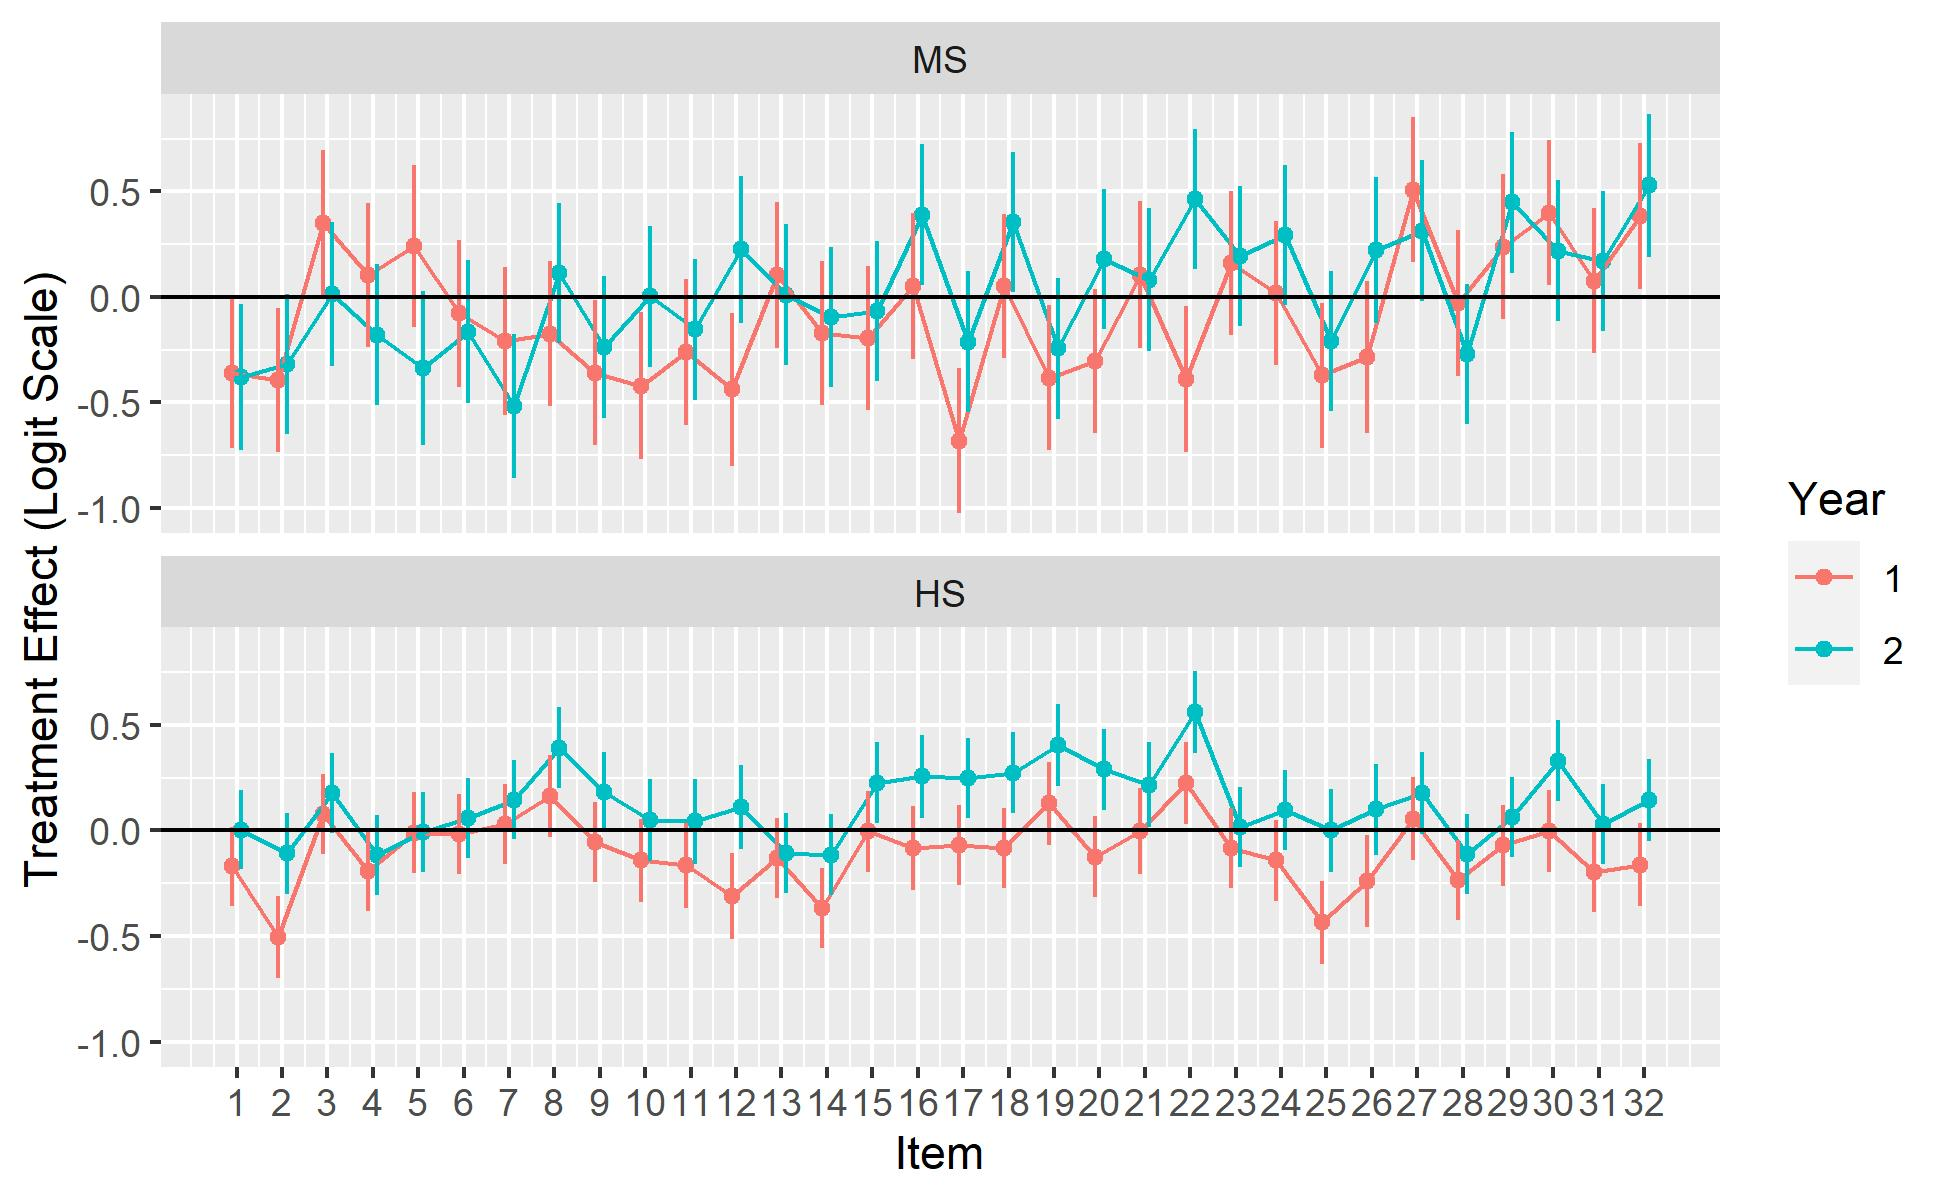
\includegraphics{../ctEffects.jpg}
  \caption{Estimated treatment effects of CTA1 for each level---high school
    or middle school---implementation year, and posttest item, with
    approximate 95\% confidence intervals}
  \label{fig:cta1Results1}
\end{figure*}


Figure \ref{fig:cta1Results1} gives the results from model
\eqref{eq:cta1model} fit to the middle school and to the high school
sample.
Each point on the plot represents the estimated effect of assignment
to the CTA1 condition on the log odds of a correct answer on one
posttest item.
The estimates are accompanied by approximate 95\% confidence
intervals.

It is immediately clear that the effect of assignment to CT vary
between posttest items--indeed the $\chi^2$ likelihood ratio test
rejects the null hypothesis of no treatment effect variance with
$p<0.001$ in all four strata.

In the middle school sample, the average treatment effect across items
was close to 0 for both years (-0.08 in year 1 and 0.03 in year 2 on
the logit scale), and not statistically significant.
However, the standard deviation of treatment effects between problems
was much higher---0.31 in year 1 and 0.29 in year 2, implying that
assignment to CTA1 boosted performance on some problems and hurt
performance on others.
To interpret the standard deviation of effects on the probability
scale, consider that for a marginal student, with a 1/2 probability of
answering an item correctly, a difference of 0.3 between two treatment
effects would correspond to a difference in the probability of a
correct answer of about 7.5\% (using the ``divide by 4 rule'' of
\cite{gelmanHill} p. 82).
The effects are also moderately correlated across the two years, with
$\rho\approx 0.4$---items that CTA1 impacted in year 1 were somewhat
likely to be similarly impacted in year 2.

Many of the treatment effects in the upper pane of Figure
\ref{fig:cta1Results1} are estimated with too much noise to draw strong
conclusions---the sample size was substantially smaller in the middle
school stratum than in the high school stratum.
However, some effects are discernible: in year 1, effects were
negative, and on the order of roughly 0.4 on the logit scale (0.1 on the
probability scale for a marginal student) on items 1, 2, 9, 10, 12,
19, 22, and 25, and on the order of approximately 0.7 for item 17
(which asks students to match a linear equation to its graph), and
similarly-sized positive effects on items 27, 30, and 32.
In year 2 there were fewer clearly negative effects---on items 1 and
7---and more positive effects, such as on items 16, 18, 22, 29, and 32. 
There is a striking difference between the year 1 and year 2 effects
on item 22, which asks students to match a quadratic expression to its
graph---the effect was quite negative in year 2 and quite
positive in year 2.

In the high school sample, the average treatment effect across items
was roughly -0.1 in year 1 and 0.13 in year 2, on the logit scale,
neither statistically significant--though the difference between the
average effect in the two years was significant ($p<0.001$).
The effects varied across items, though less widely in high school
than in middle school---in both years the standard deviation of
item-specific effects was roughly 0.17.
Item-specific effects were more highly correlated across years
($\rho\approx 0.69$)---at some points in the lower pane of Figure
\ref{fig:cta1Results1} it appears as though the curve from year 2 was
simply shifted up from year 1.

The item-specific effects in the high school sample were estimated
with substantially more precision than in the middle school sample,
due to a larger sample size.
In year 1, there were striking negative effects on items 2, 14, and 25
which ask students to manipulate algebraic expressions, and on item
12, which ask students to calculate the length of the side of a
triangle. In year 2, these negative effects disappeared. Instead,
there were positive effects, especially on items 8 and 22, which both
ask about graphs of algebraic functions, and on a stretch of items
from 15--22. The difference in the estimated effects between years was positive
for all items and highest
for problems 2, 20, and 25, which ask students to manipulate or
interpret algebraic expressions, and 12, the triangle problem. In
items 2, 12, and 25, the effect was significantly negative in year 1
and closer to zero in year 2, while for item 20 the effect was close
to zero in year 1 and positive in year 2. 

\begin{figure*}
  \centering
  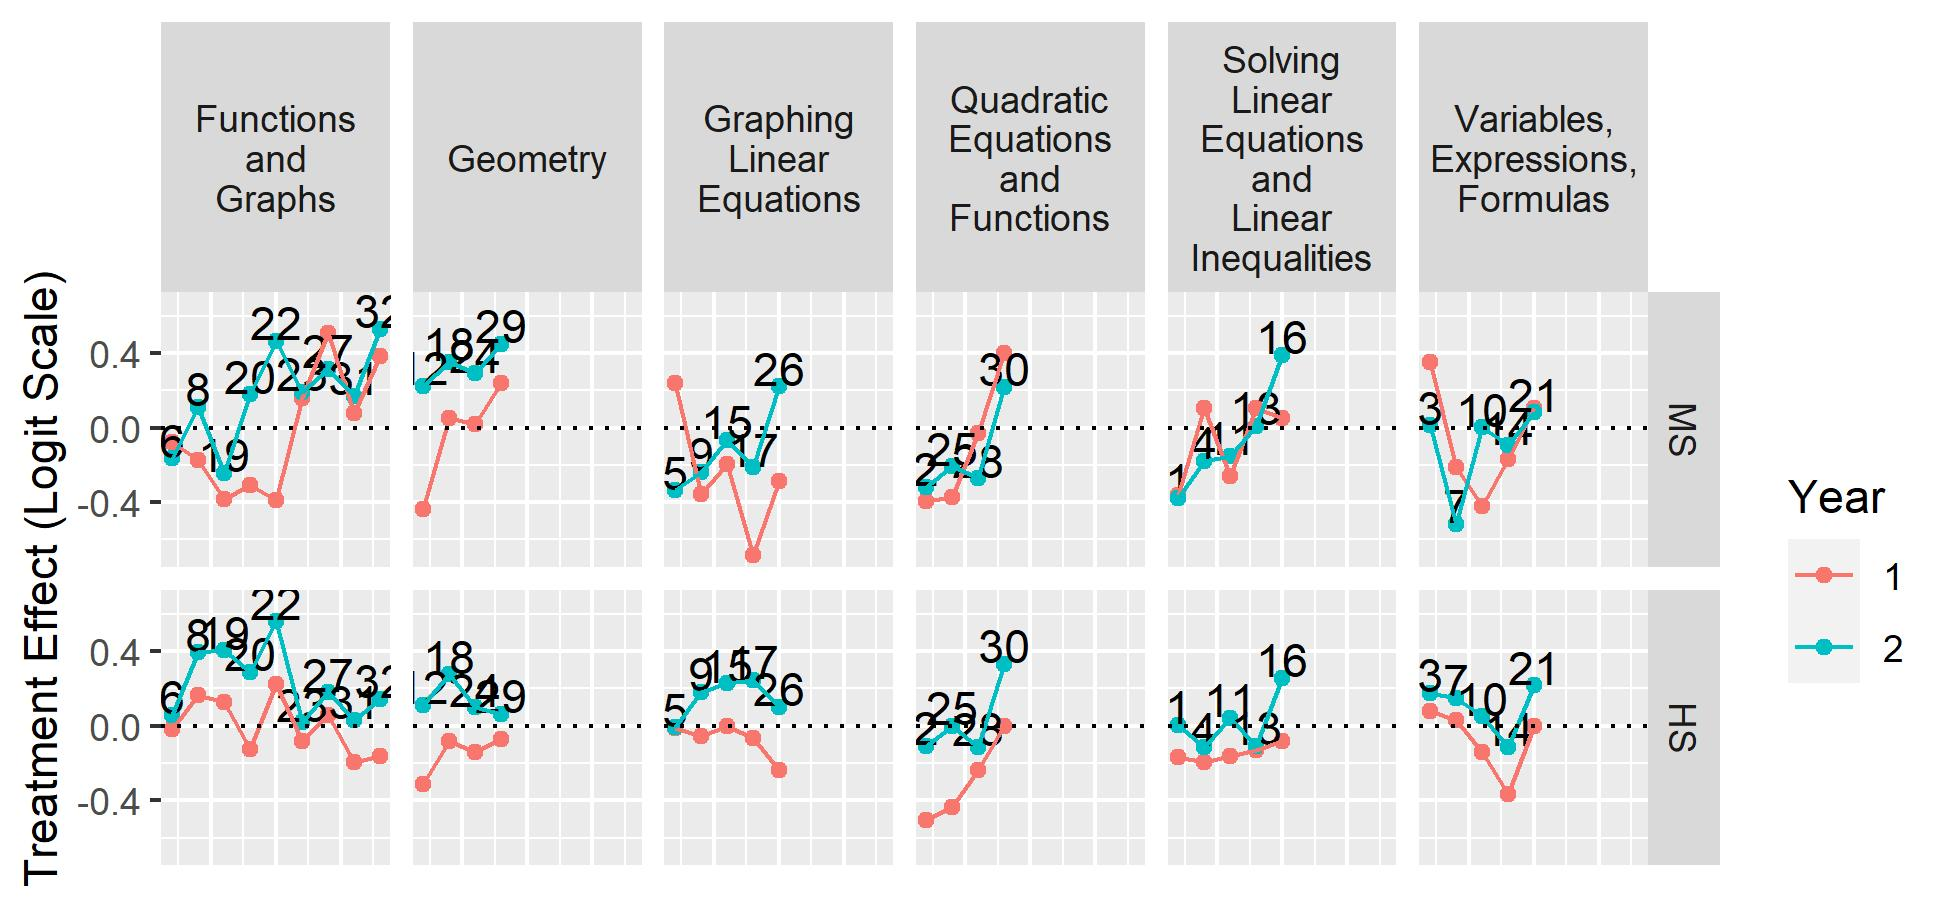
\includegraphics{../ctEffectsType.jpg}
  \caption{Estimated treatment effects of CTA1 posttest items arranged
    by the group of skills each item is designed to test. See Table
    \ref{tab:ctSkills} for more detail.}
  \label{fig:cta1ResultsType}
\end{figure*}

Figure \ref{fig:cta1ResultsType} plots the estimated effect on each
posttest item as a function of the item's objective in Table
\ref{tab:ctSkills}.
Some patterns are notable.
There was a wide variance in the effects on the four geometry problems
for middle schoolers in year 1, but in year 2 all the effects on
geometry items were positive and roughly the same size.
The geometry items in the high school sample follow a similar, if less
extreme, pattern.
Across both middle and high school, the largest positive effects were
for Functions and Graphs problems, especially item 22 for year 2; on items 23,
27, 31 and 32, middle schoolers---especially in year 2---saw positive
effects while high schoolers saw effects near 0.

\subsection{ASSISTments}
\begin{figure*}
  \centering
  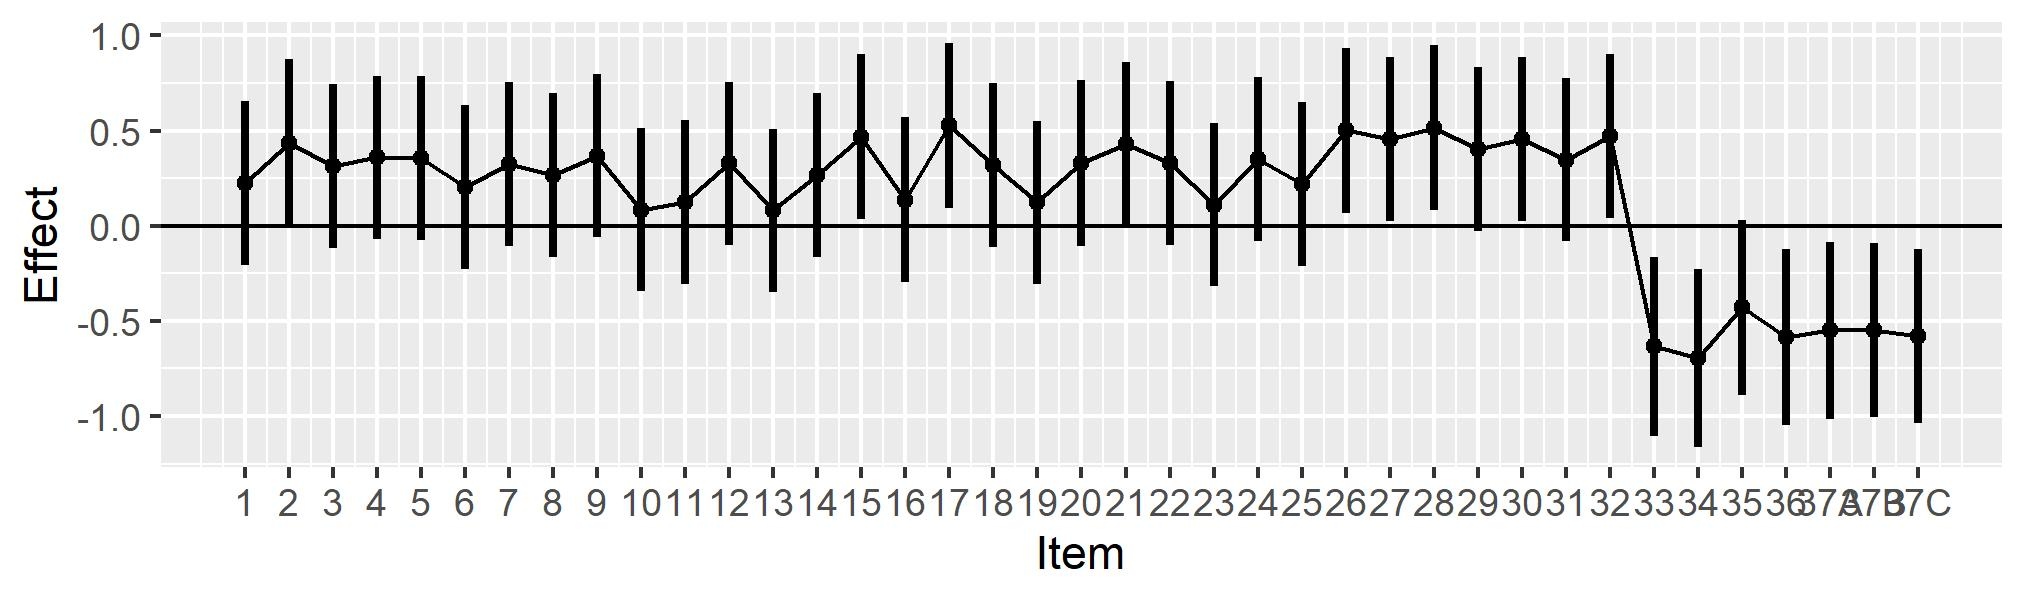
\includegraphics{../assEffects.jpg}
  \caption{Estimated treatment effects of ASSISTments for each posttest item, with
    approximate 95\% confidence intervals}
  \label{fig:assResults1}
\end{figure*}

Figure \ref{fig:assResults1} gives the results from model
\eqref{eq:assmodel}, plotting item-specific effect estimates with
approximate 95\% confidence intervals for each TerraNova posttest
item.
It is immediately apparent that there were a negative effects on
open-ended questions, 33--37C, and (somewhat more ambiguous) positive
effects on multiple choice items.
The model estimated an average effect of 0.32, with a standard error
of 0.20, for multiple choice problems, and of -0.52, with a standard
error of 0.21, for open-ended questions.
After accounting for that difference (i.e. within item type
categories) the standard deviation of item-specific effects was positive
(p<0.001) but less than for the CTA1 items: it was estimated as 0.15
on the logit scale.
The confidence intervals in Figure \ref{fig:assResults1} are also much
wider than those for CTA1; we suspect that a large part of the reason
is that we did not have access to pretest scores, an important
covariate.

The largest effects on the multiple choice items were 28 and 17, which both
required students to plug in values for variables in algebraic
expressions. The confidence intervals around the effects for items 15,
26, 27, 30, and 32 also exclude 0.
On the other end, effects on all open-ended items other than 35 were
statistically significant, and fairly similar to each other. 

\begin{figure*}
  \centering
  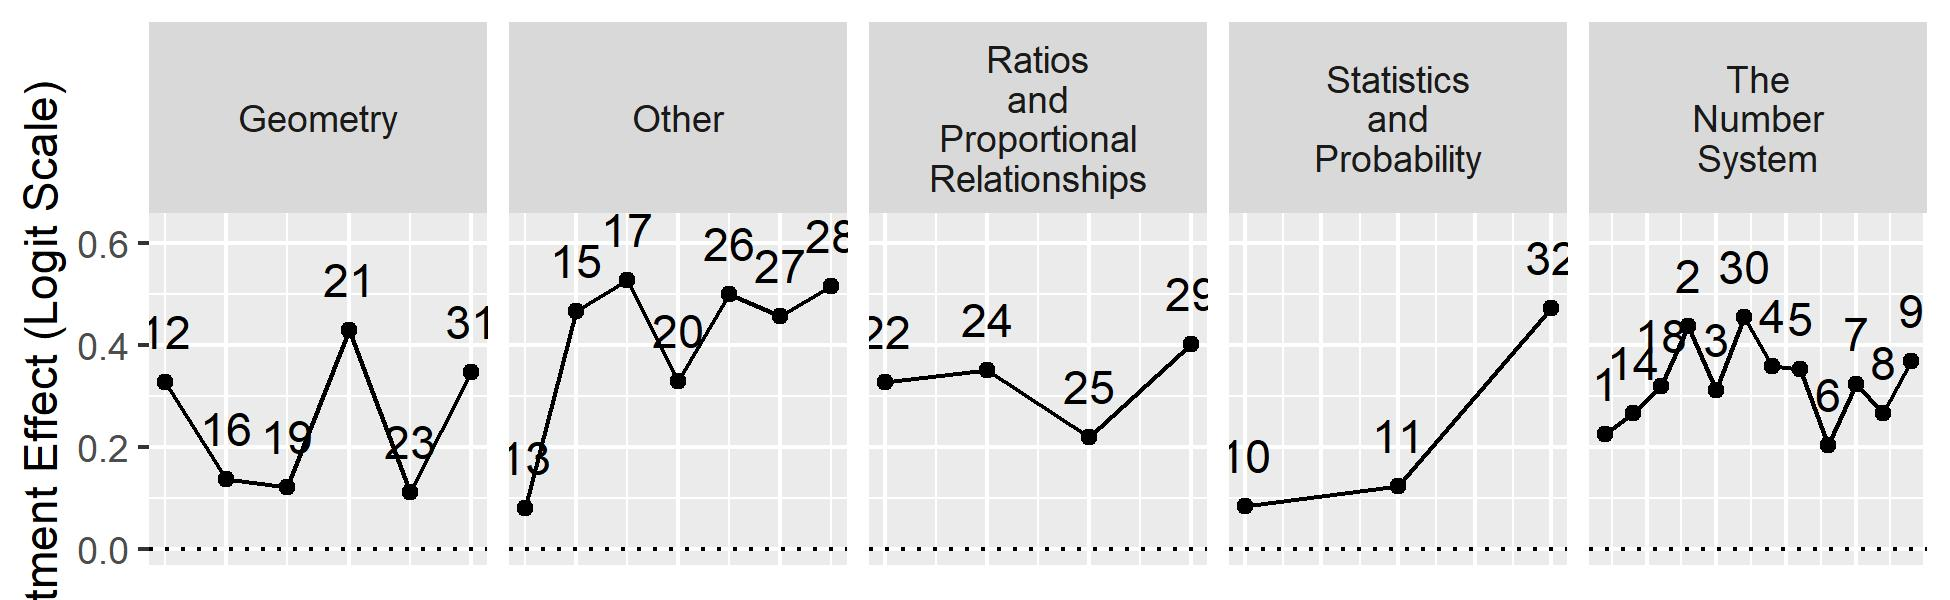
\includegraphics{../assEffectsType.jpg}
  \caption{Estimated treatment effects of ASSISTments for each
    multiple choice
    posttest item, arranged according to CCSS, as in Table
    \ref{tab:assistmentsSkills}. The ``Other'' category includes
    Functions and the two Mathematical Practice standards, ``make
    sense of problems and persevere in solving them'' and ``reason
    abstractly and quantitatively''.}
  \label{fig:assResults2}
\end{figure*}

Figure \ref{fig:assResults2} plots item-specific effects for multiple
choice TerraNova items grouped according to their CCSS, as in Table
\ref{tab:assistmentsSkills}, with the non-grade-7 standards grouped
together as ``Other.''
Interestingly, the largest effects tended to be for items in this
``Other'' category---as did the smallest effect, for item 13.
Effects for problems in the ``Number System'' and ``Ratios and
Proportional Relationships'' categories had the most
consistent effects, between 0.2 and 0.4 on the logit scale. 

\section{Exploring Hypotheses about \emph{Why} ASSISTments Effects Differed}\label{sec:hypotheses}
Researchers on the ASSISTments team have built on the CCSS links of
Table \ref{tab:assistmentsSkills}, linking TerraNova posttest items to
data on student work within ASSISTments, for students in the treatment
condition.
This gives us an opportunity to use student work within ASSISTments to
explain some of the variance in treatment effects.

Like TerraNova items in Table \ref{tab:assistmentsSkills}, ASSISTments
problems are linked with CCSS.
By observing which problems treatment students worked on, and using this
linkage, we could observe which Common Core standards they worked on
the most within ASSISTments.
We hypothesized that treatment effects might be largest for the
TerraNova problems that were linked with the Common Core standards
students spent the most time working on.
In other words, we linked TerraNova items with worked ASSISTments
problems \emph{via} Common Core standards.
The Common Core linkage we used in this segment was finer-grained than
Table \ref{tab:assistmentsSkills}, so TerraNova items in the same
category in Table \ref{tab:assistmentsSkills} may not be linked with
the same problems in this analysis.

We examined our hypothesis in two ways: examining the relationships
between treatment effects and the number of related ASSISTments
problems students in the treatment group worked, and the number of
related ASSISTments problems students in the treatment group worked
\emph{correctly}. 
This analysis includes two important caveats: first, the linkages,
both between TerraNova items and CCSS, and between ASSISTments
problems and CCSS, were subjective and error-prone, possibly
undermining the linkage between TerraNova items and ASSISTments
problems. 
Secondly, student work in ASSISTments is necessarily a post-treatment
variable---it was affected by treatment assignment.
If the treatment randomization had fallen out differently, different
schools would have been assigned to the ASSISTments condition and
different ASSISTments problems would have been worked.
Including the number of worked or correct related problems as a
predictor in a causal model risks undermining causal interpretations
\cite{montgomery2018conditioning}.

\begin{figure*}
  \centering
  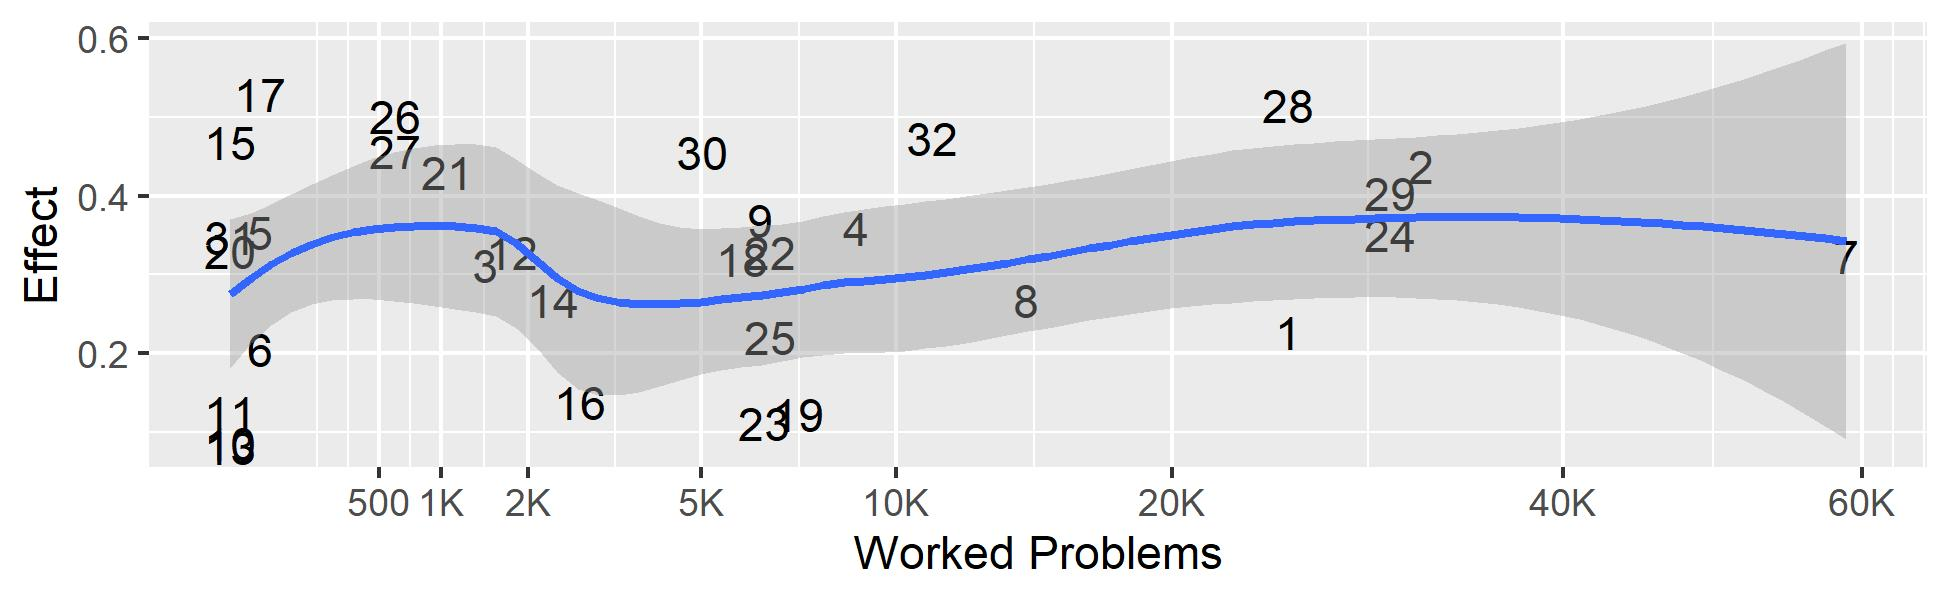
\includegraphics{../assEffectsWorkedProbs.jpg}
  \caption{Estimated effects on multiple-choice TerraNova items
    plotted against the number of related ASSISTments problems that
    students in the treatment arm worked over the course of the
    study. The X-axis is plotted on the square-root scale, and a
    non-parametric loess fit is added for interpretation.}
  \label{fig:workedProbs}
\end{figure*}

\begin{figure*}
  \centering
  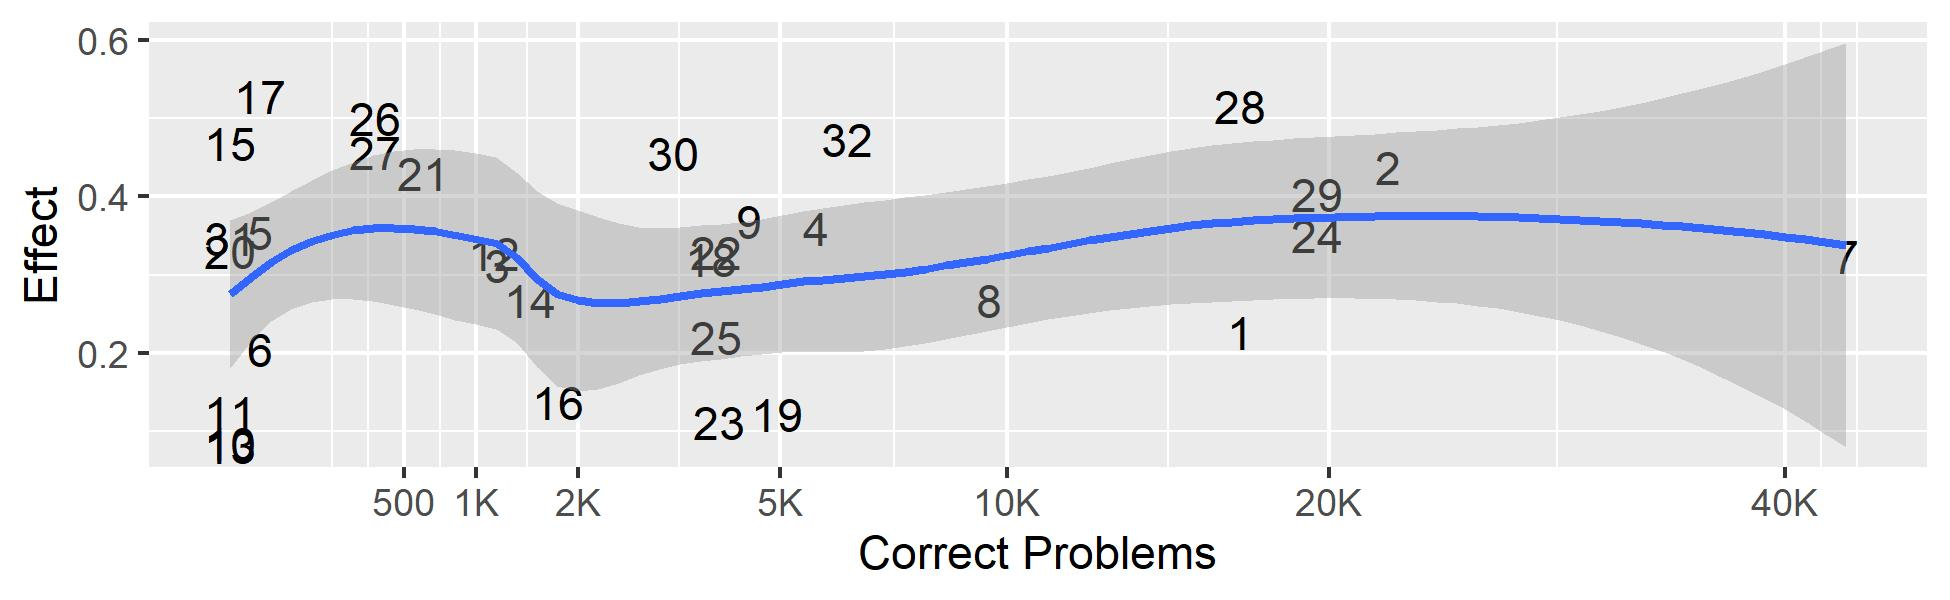
\includegraphics{../assEffectsCorrectProbs.jpg}
  \caption{Estimated effects on multiple-choice TerraNova items
    plotted against the number of related ASSISTments problems that
    students in the treatment arm worked correctly over the course of the
    study. The X-axis is plotted on the square-root scale, and a
    non-parametric loess fit is added for interpretation.}
  \label{fig:correctProbs}
\end{figure*}


Figures \ref{fig:workedProbs} and \ref{fig:correctProbs} plot
estimated item-specific effects for multiple choice TerraNova items against the number of ASSISTments
problems that students in the treatment arm worked or worked
correctly, respectively, over the course of the RCT.
The X-axis is on the square-root scale, and a loess curve is added for
interpretation. 
Little, if any, relationship is apparent in either figure, suggesting
either the lack of a relationship between specific ASSISTments work
and posttest items, or issues with the linkage.
This is hardly surprising, given both the difficulty in linking
ASSISTments and TerraNova problems, and given the fact that topics in
mathematics are inherently connected, so that improving one skill
tends to improve others as well.


\section{Conclusions}\label{sec:conclusion}

Education researchers are increasingly interested in ``what works.''
However, the effectiveness of an intervention is necessarily
multifaceted and complex---effects differ between students, as a
function of implementation \cite{sales2016student}, and, potentially,
as a function of time and location.
In this paper we explored a different sort of treatment effect
heterogeneity---differences in effectiveness for different
outcomes---specifically, different posttest items measuring different
skills.
Collapsing item-level posttest data into a single test score has the
advantage of simplicity (which is nothing to scoff at, especially in
complex causal scenarios) but at a cost.
Analysis using only summary test scores squanders a potentially rich
source of variability and information about intervention effectiveness
that is already at our fingertips.
There is little reason \emph{not} to examine item-specific effects.

In this paper, we showed how to estimate item specific effects using a
Bayesian or empirical Bayesian multilevel modeling approach that, we
argued, can improve estimation precision and avoid the need for
multiplicity corrections.
The estimates we provided here combine maximum likelihood estimation
and empirical Bayesian inference; there is good reason to suppose that
a fully Bayesian approach would provide greater validity, especially
in standard error estimation and inference.
However, fitting complex multilevel models using Markov Chain Monte
Carlo methods is computationally expensive, and can be very slow, even
with the latest software.
We hope to explore this option more fully in future work.

While estimating item-specific effects is relatively straightforward,
interpreting them presents a significant challenge.
This is due to a number of factors: first, when looking for trends in
treatment effects by problem attributes, the sample size is the number
of exam items, not the number of students, so patterns can be hard to
observe and verify.
Secondly, there is a good deal of ambiguity and subjectivity involved
in defining and determining item attributes and features, which is
exacerbated by the fact that standardized tests generally cannot be
made publicly available.
Lastly, since student ITS work over the course of a study is
necessarily post-treatment assignment, careful causal modeling (such
as principal stratification \cite{sales2016student}) may be necessary.
Examining heterogeneity between item-specific treatment effects may
play a larger role in helping to generate hypotheses about ITS
effectiveness than in confirming hypotheses.

Despite those difficulties, the analysis here uncovered important
information about the CTA1 and ASSISTments effects.
First, the discovery that the effects vary between items is notable in
itself. 
In our analysis of CTA1 we noticed that some of the largest
effects---and differences between first and second-year effects---
were for posttest items involving manipulating algebraic expressions
and interpreting graphs.
In our analysis of ASSISTments, we discovered a large difference
between negative effects on open-ended questions and positive effects
on multiple choice questions, and also that the largest effects were
on problems requiring students to plug numbers into algebraic
expressions.

We hope that this research will serve as a proof-of-concept and spur
further work delving deeper into data we already have.

\bibliographystyle{abbrv}
\bibliography{bib,ct}  % sigproc.bib is the name of the Bibliography in this case

\appendix

\section{A Simulation Study of Multiple Comparisons}
We ran a small simulation study testing \cite{gelman2012we}'s
assertion that multiplicity corrections are unnecessary when
estimating different effects from BLUPs in a multilevel model.
\cite{gelman2012we} stated their case in terms of fully Bayesian
models, whereas we used an empirical Bayesian approach that may differ
somewhat.

In our simulation, in each simulation run, we generated data on
$Nexpr$ experiments, where $Nexpr$ was a parameter we varied.
In each experiment, there were $n=500$ simulated subjects, half assigned to
treatment and half to control. They were given ``outcome'' data $Y\sim
N(0,1)$, with no treatment effect.

We analyzed the experiment data in two ways. First, we estimated a
p-value for each experiment separately, using t-tests. This is the
conventional approach. Then, we we estimated a multilevel model:
\begin{equation*}
  Y_{ij}=\beta_0+\gamma_{1j}Expr_j+\gamma_{2j}Trt_i+\epsilon_{ij}
\end{equation*}
where $\beta_0$ is an intercept, $\gamma_{1j}$ are random intercepts
for experiment, $\gamma_{2j}$ is the treatment effect for experiment
$j$, and $\epsilon_{ij}$ is a normally-distributed error term.
$\bm{\gamma}\sim MVN\left(\{0,\gamma_{20}\},\Sigma\right)$ where
$\gamma_{20}$ is the average effect across all experiments.
The number of experiments in each simulation run, $Nexpr$, was varied from 5 to
40, in increments of 5.
In each case, we estimated the familywise error rate, the probability
of at least one statistically significant effect estimate (at
$\alpha=0.05$) across the
$Nexpr$ experiments.

The results are in Figure \ref{fig:sim}.
As expected, the familywise error rate increased rapidly when effects
were estimated and tested separately in each of the $Nexpr$
experiments.
When effects were estimated jointly in a multilevel model, in a way
analogous to the method described in Section \ref{sec:method}, the
familywise error rate remained roughly constant as $Nexpr$ increased.
However, the familywise error rate in the multilevel modeling approach
was slightly elevated, ranging from roughly $0.05$ to $0.075$.

\begin{figure}
  \centering
  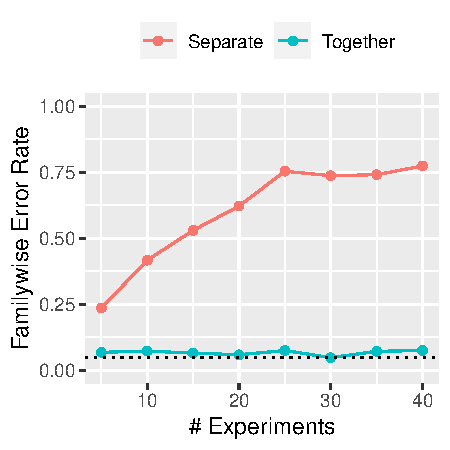
\includegraphics[width=0.45\textwidth]{../simulationResults}
  \caption{United we stand: results from a simulation of familywise
    error rate using separate t-tests for each experiment or using
    multilevel modeling.}
  \label{fig:sim}
\end{figure}

\end{document}
